\documentclass[a4paper]{report}
\usepackage{amsmath,amssymb,booktabs,bm,caption,enumerate,float,geometry,graphicx,indentfirst,setspace,titlesec}
\geometry{left=4.5cm,right=4.5cm,top=4cm,bottom=4cm}
\captionsetup[figure]{labelsep=period}
\begin{document}
	\renewcommand\thesection{\arabic{section}}
	\begin{Large}
		\begin{center}
			\setlength{\baselineskip}{14pt}
			\vspace{1.25cm}
			\rule[0cm]{11.2cm}{0.03em}\\
			\vspace{0.5cm}
			\textsc{UM-SJTU Joint Institute}\\
			\vspace{0.25cm}
			\textsc{Physics Laboratory\\(Vp141)}
			\vspace{0.3cm}
			\rule[0cm]{11.8cm}{0.05em}
			\vspace{4.9cm}\\
			\textsc{Laboratory Report}
		\end{center}
	\end{Large}
	\vspace{0.85cm}
	\begin{large}
		\begin{center}
			\textsc{Exercise 4}
			\\~
			\textsc{Measurement of the Speed of Sound}
		\end{center}
		\vspace{6cm}
	\end{large}
	\begin{tabular}{l l l}
	Name: Yihua Liu&ID:518021910998&Group 9\\
	Name: Guanghan Xi&ID:518021910778&Group 9\\
	&&\\
	Date: 21 June 2019&&\\
	\end{tabular}
	\thispagestyle{empty}
	\newpage
	\section{Introduction}
	The Objective of the exercise is to experiment on the damped and driven oscillations both with the Pohl resonator. Besides, we will observe and quantify the phenomenon of the mechanical resonance further as for the driven oscillations.
	
	If the amplitude of the resonance system decreases gradually due to friction or medium resistance or other energy consumption, the resonance is called damped oscillation. Denote the damping coefficient as $b$ and the stiffness as $k$, we have
	\begin{equation}
	m\dfrac{d^2x}{dt^2}+b\dfrac{dx}{dt}+kx=0
	\end{equation}
	Solving the differential equation, if $b^2<4km$, it is an underdamped regime
	\begin{equation}
	x(t)=Ae^{-\frac{b}{2m}t}\cos{(\sqrt{{\omega_0}^2-\dfrac{b^2}{4m^2}}t+\varphi)}
	\end{equation}
	If $b^2>4km$, it is an overdamped regime
	\begin{equation}
	x(t)=C_1e^{-(\frac{b}{2m}+\sqrt{\frac{b^2}{4m^2}-(\omega_0)^2})t}+C_2e^{-(\frac{b}{2m}-\sqrt{\frac{b^2}{4m^2}-(\omega_0)^2})t}
	\end{equation}
	If $b^2=4km$, it is a critical regime
	\begin{equation}
	x(t)=(D_1+D_2t)e^{-\frac{b}{2m}t}
	\end{equation}
	If a periodic force exerts on a resonance system, the resonance is called forced or driven oscillation. For a system endowed with single degree of freedom, the driving force has the form
	\begin{equation}
	F=F_0\cos{\omega t}
	\end{equation}
	where $F_0$ is the amplitude and $\omega$ is the angular frequency. Then, the kinetic motion for the linear driven oscillation can be written in the form of derivatives:
	\begin{equation}
	m\frac{d^2x}{dt^2}=-b\frac{dx}{dt}-kx+F_0\cos{\omega t}
	\end{equation}
	
	In this experiment, we study a rotating system instead of a translational system that the kinetic equation can be rewriten as
	\begin{equation}
	I\frac{d^2\theta}{dt^2}=-k\theta -b\frac{d\theta}{dt}+\tau_0\cos{\omega t}
	\end{equation}
	where $I$ is the moment of intertia, $\tau_0$ is the amplitude, $\omega$ is the angular frequency. The second item is the damping torque and the third item is the periodic driving torque.
	
	Drawing an analogy between the translational motions and rotating motions, we simplify the equation by
	\begin{equation}
	\omega_0^2=\frac{k}{I},\qquad 2\beta=\frac{b}{I},\qquad \mu=\frac{\tau_0}{I},
	\end{equation}
	Eq. (7) can be rewritten as
	\begin{equation}
	\frac{d^2\theta}{dt^2}+2\beta\frac{d\theta}{dt}+\omega_0^2\theta=\mu\cos{\omega t}
	\end{equation}
	
	Consider a critical condition that the driving torque $\mu=0$, the equation can express the motion for a damped harmonic oscillator. Another critical condition is that the damping in the system $\beta=0$ so that it becomes a simple harmonic oscillator with $\omega_0$, the natural angular frequency.
	
	Seperating the transient term $\theta_tr$ and the steady-state term $\theta_st$ from the time function of the angle $\theta(t)$,
	\begin{equation}
	\theta(t)=\theta_{tr}(t)+\theta_{st}\cos{\omega t+\varphi}
	\end{equation}
	
	Analyze the differential equation quantitatively, the trasient solution $\theta_{tr}$ decrease to 0 exponentially as $t\rightarrow\infty$. On the other hand, the steady-sate solution $\theta_{st}$ multiplied by cosine function is endowed with the amplitude
	\begin{equation}
	\theta_{st}=\dfrac{\mu}{\sqrt{(\omega_0^2-\omega^2)+4\beta^2\omega^2}}
	\end{equation}
	The lags $\varphi$ from the equilibrium position to the position when time is $t$ in the form of the tangent of phase shift is
	\begin{equation}
	\tan{\varphi}=\frac{2\beta\omega}{\omega^2-\omega_0^2},
	\end{equation}
	where $-\pi\leq\varphi<0$. Different from the transient term $\theta_{tr}$, both the amplitude and the phase shift are not determined by the initial conditions.
	
	Looking for the maximum value of $\theta_{st}$ as a function of $\omega$, the resonance angular frequency is
	\begin{equation} \omega_{\rm{res}}=\omega=\sqrt{\omega_0^2-2\beta^2}
	\end{equation}
	Substitute $\omega$ into Eq.11, the amplitude of the resonance angle is
	\begin{equation}
	\theta_{\rm{res}}=\theta_{st}(\omega_{\rm{res}})=\frac{\mu}{2\beta\sqrt{\omega_0^2-\beta^2}}
	\end{equation}
	
	When the damping coefficient $\beta\rightarrow0$, the resonance angular frequency $\omega_{\rm{res}}\rightarrow\omega_0$. Under this circumstance, the amplitude of the steady-state oscillations is close to its maximum value. Taking different values of $\beta$ that $\beta_1>\beta_2>\beta_3$ for comparing the amplitude $\theta$ related to the ratio $frac{\omega}{\omega_0}$ and $\beta_1<\beta_2$ for comparing the phase shift  $\varphi$ related to $frac{\omega}{\omega_0}$ in Figure 1.
	\begin{figure}[H]
		\centering
		\includegraphics[width=1\linewidth]{1.jpg}
		\caption{The dependence of the amplitude (left) and phase shift (right) of steady-state driven oscillations [1].}
	\end{figure}
	Looking for the homogeneous equation of Eq. (9) conditioned initally by $\theta(t)=\theta_0e^{-\beta t}\cos{(\omega_{\rm f} t+\alpha)}$, we have $\theta_1=\theta_0e^{-\beta T},\theta_2=\theta_0e^{-\beta(2T)},...,\theta_n=\theta_0e^{-\beta(nT)}$. Hence, the damping coefficient $\beta$ is
	\begin{equation}
	\ln{\frac{\theta_j}{\theta_i}}=\ln{\frac{\theta_0e^{-\beta(iT)}}{\theta_0e^{-\beta(jT)}}}=(j-i)\beta T
	\end{equation}
	where we can calculate the damping coefficient $\beta$ by the period $T$.
	\section{Experimental setup}
	The BG-2 Pohl resonator is mainly composed by a vibrometer and a control box. The vibrometer is shown in Figure 2.
	\begin{figure}[H]
		\centering
		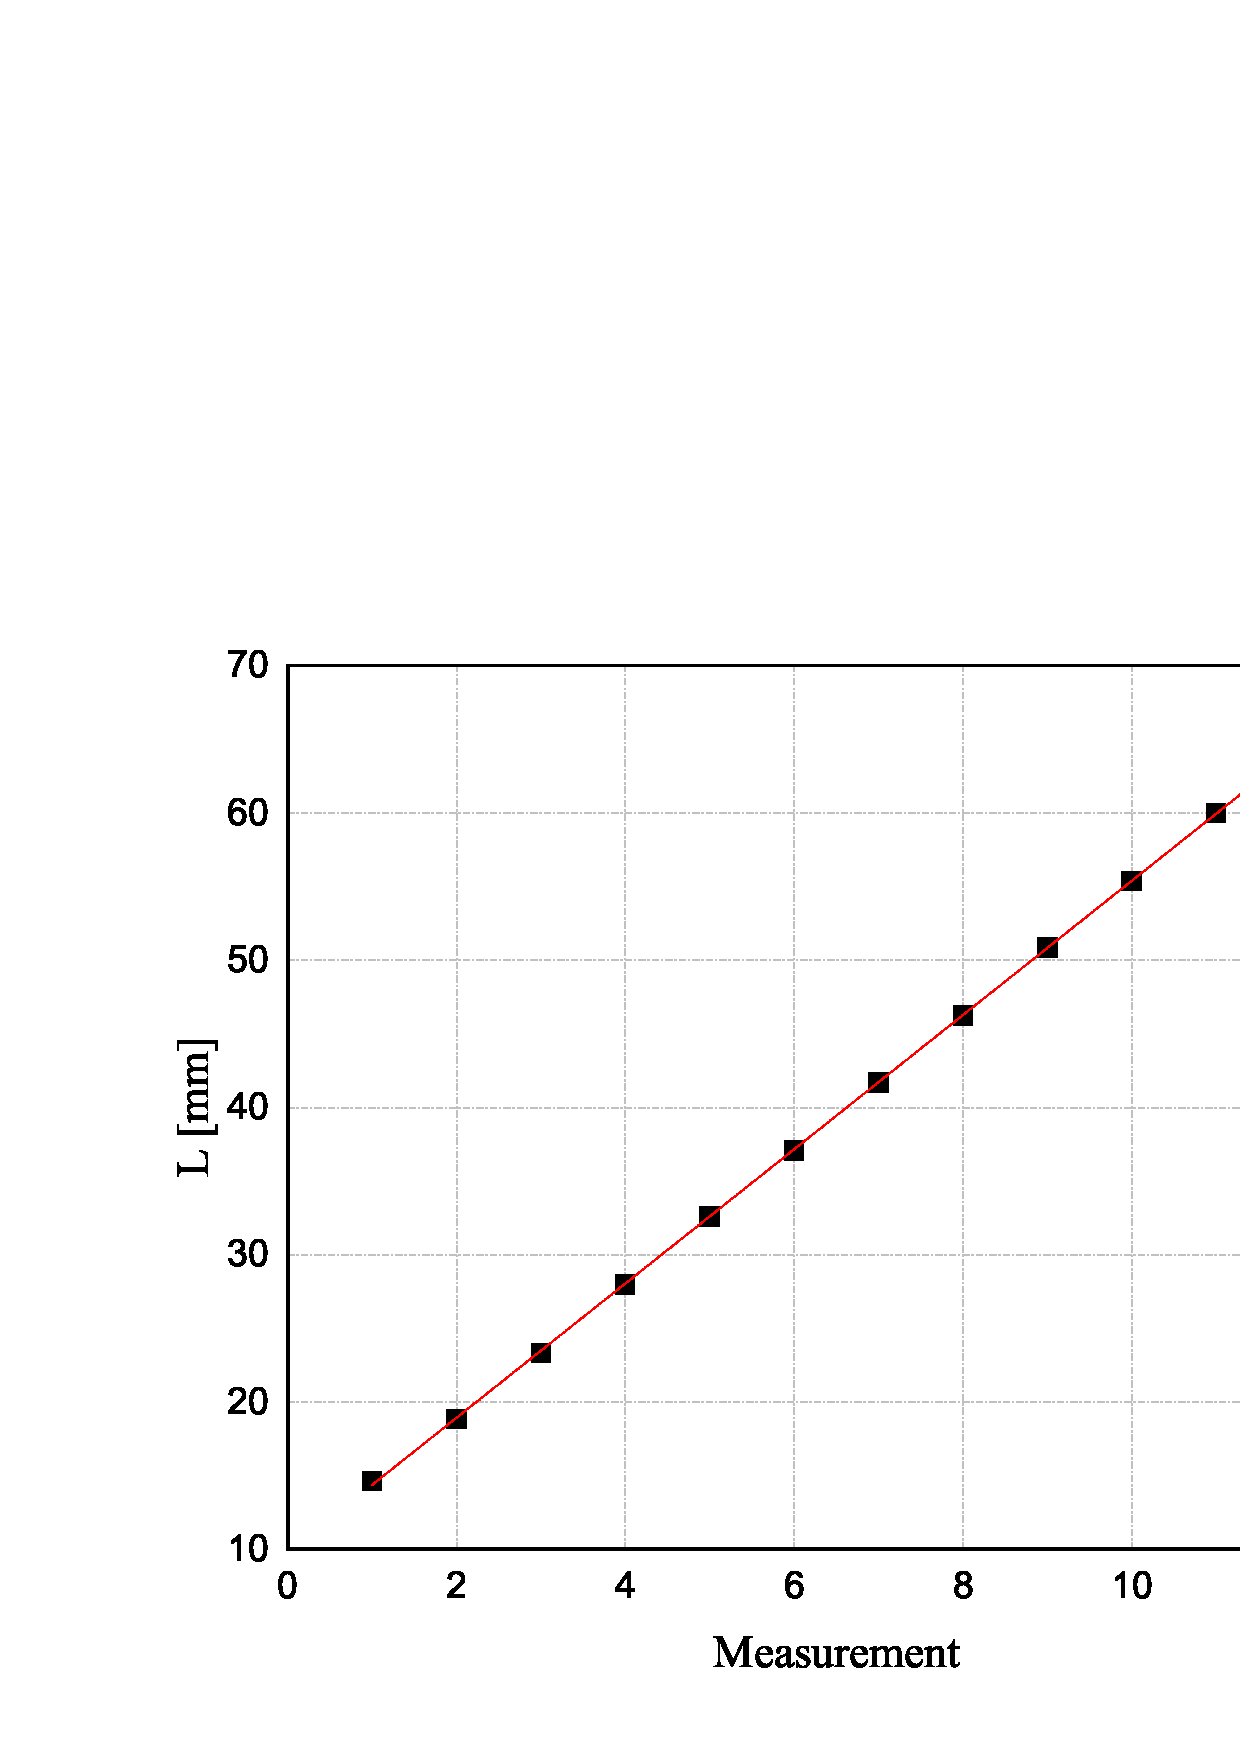
\includegraphics[width=1\linewidth]{2.jpg}
		\caption{The vibrometer [2].}
	\end{figure}
	The equipment is supported by the balance wheel. The spring mounted on the supporting frame is to provide an elastic restoring torque to the wheel that is attached to it. At the equilibrium position, the balance whell will rotate. The notches on the edge of the balance whell. Some are shallow while one of them is deep that is used to set a photoelectric detector. The detector connected to the electronic control box can measure the amplitude and the period of an 
	oscillation.
	
	At the bottom of the supporting frame on the pedestal, a pair of coils are configured and the balance wheel fit well into the gap between them, connected by adjustment screws. The mechanism of the electromagnetic damping force is the electromagnetic induction. Changing the current carried by the pair of coils, the magnitude of the damping force changes. On the right side, a motor is used to drive the eccentric whell with a rod.
	
	The electric control box that can control the speed of the motor precisely is shown in Figure 3.
	\begin{figure}[H]
		\centering
		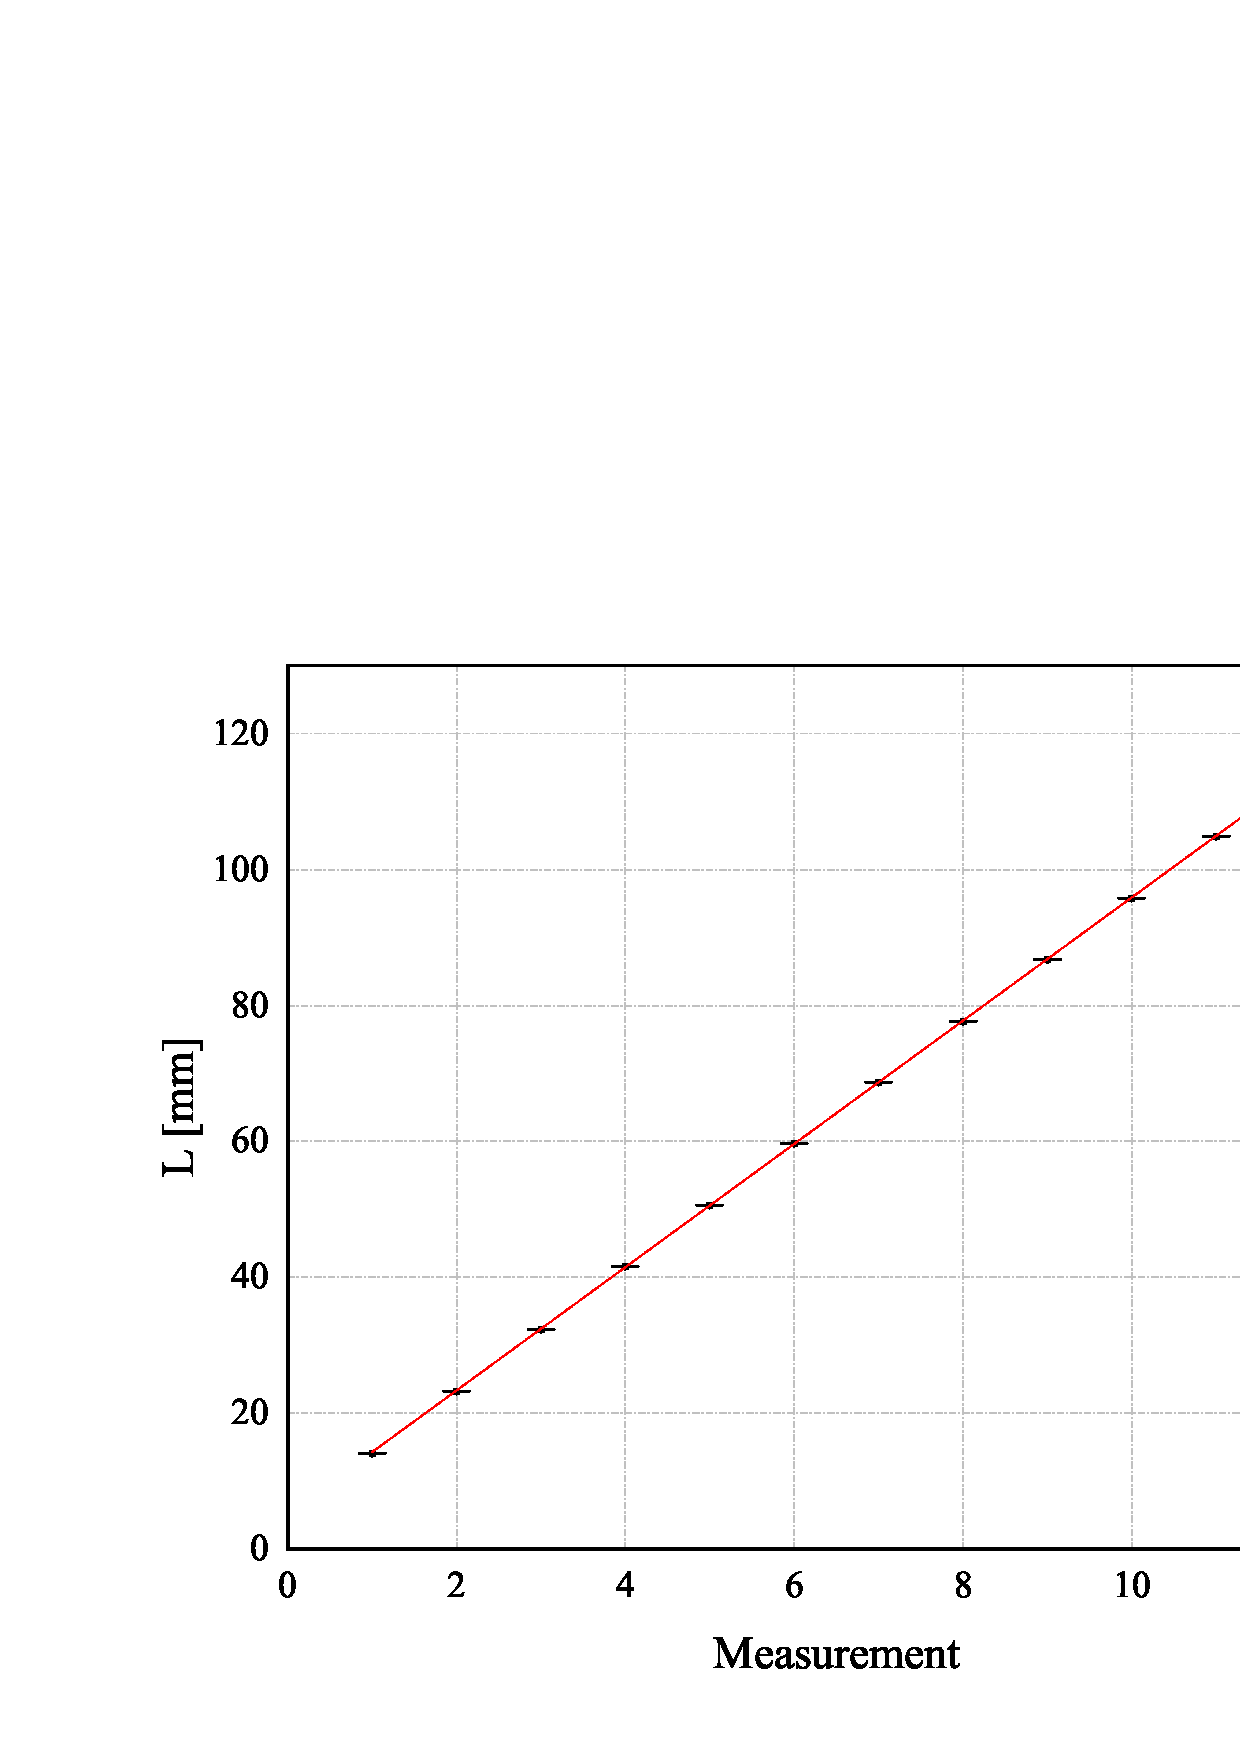
\includegraphics[width=1\linewidth]{3.jpg}
		\caption{The front panel of the control box [3].}
	\end{figure}
	The electric control box provides 8 options on the front panel. The function \textsf{Amplitude Display} can display the amplitude of the balance wheel. \textsf{Period Display} can display the period of the oscillation in two modes. \textsf{Period Selection} can switch two periods of the oscillation, "1" meaning single and "10" meaning the time of 10, the latter one used in this experiment.
	
	The knob \textsf{Period of the driving force} can precisely change the period of the driving force. \textsf{Motor Switch} switches the status of motor, in "off" when measuring the damping coefficient and the natural angular frequency. The knob \textsf{Damping Selection} can switch the level of the damping force by adjusting the current in the coils at the bottom of the balance wheel, ranging from "0" (no current) to "5" (current of around 0.6 A), 6 options in total, of which "2", "3", and "4" used in this experiment. The strobe can generate a flash according to the phase difference in angle scale to read the time period.
	\section{Measurement}
	\subsection{Natural Angular Frequency}
	Before doing experiments, we check the position of the photoelectric gate above the balanced wheel that there is enough space between them.
	
	We first turn the \textsf{Damping Selection} knob to "0". Then, we carefully rotate the balance wheel to the initial angular position $\theta_0\approx150^\circ$. Then, we release it and record the time of 10 periods. We repeat for four times and calculate the natural angular frequency $\omega_0$.
	
	At first, we mistook the initial angle as approximately 120$^\circ$ and we found that the readings of the time of 10 periods slightly changes. Hence, it is important to keep the initial angles of each time of measurement almost the same to minimize errors.
	\subsection{Damping Coefficient}
	We first turn the \textsf{Damping Selection} knob to "2", and keep it unchanged during this part. Then, we rotate the balance wheel to the initial angle of about 150$^\circ$ carefully. Then,we release it and record the angle of each period that is the amplitude and time of 10 periods. Since when the vibrometer may release the first reading before or after the copper balance wheel reaches the endpoint, we dismiss the first reading and start reading from the second reading.
	
	Having recorded all required data, we start to solve the homogeneous equation of Eq. (15). Since we read the time of 10 periods, we have $j-i=5$. Then, Eq. (15) can be rewritten as
	\begin{equation}
	\beta=\frac{1}{5T}\ln{\frac{\theta_i}{\theta_{i+5}}}.
	\end{equation}
	We then obtain the value of the average period $T$ by Eq. (16).
	
	During our experiment, we did not miss any readings with our camera. However, if we miss some readings, we should repeat the measurement recording them. Besides, by repeating the measurement, our results would be more precise.
	\subsection{$\theta_{\rm{st}}$ vs. $\omega$ and $\varphi$ vs. $\omega$ Characteristics of Forced Oscillations}
	At first, we keep the \textsf{Damping Selection} at "2" and set the speed of the motor. We record the position of the motor knob in case we need to repeat the measurement. After the motor begin working and the oscillation reaches a steady state, we record the amplitude $\theta_{\rm{st}}$, the period $T$, and the phase shift $\varphi$.
	
	Then, we repeat operating the motor and recording data but change the speed of motor to change a small phase shift $\Delta\varphi$. We generally adjust the amplitude to 90$^\circ$ where there is a maximum value for it is a resonance point and to 0$^\circ$ or 180$^\circ$. In total we have more than 15 data collected for plotting.
	
	As we observe, when the amplitude is going to reach the maximum value, it changes rapidly as $\varphi$ and $\theta_{\rm{st}}$ change. Besides, when $\varphi$ and $\theta_{\rm{st}}$ reach their limit, they cannot reach the endpoint 0$^\circ$ or 180$^\circ$.
	
	Next, we can choose \textsf{Damping Selection} "1" or "3". We choose "3" and repeat steps above. We can no longer change the \textsf{Damping Selection} to ensure the accuracy of the measurement until it is entirely completed. Having collected demanding data, we plot the $\theta_{\rm{st}}(\omega)$ characteristics with $\omega/\omega_0$ on the horizontal axis and $\theta_{\rm{st}}$ on the vertical axis and two sets of data plotted together. We choose "3" partly because we find the values in previous measurement choosing "2" is large enough.
	\section{Results}
	\subsection{Natural Angular Frequency}
	The period of oscillations was measured in the procedure in section 3.1. We calculate the average value of the period $T$ according to the results in Table 1 as
	\begin{equation*}
	\bar{T}=\frac{1}{40}\sum_{i=1}^4T_i=1.5782\pm0.0003 \ \rm s
	\end{equation*}
	with the relative uncertainty 0.02\%.
	\begin{center}
	\begin{tabular}{|c|c|}
		\hline
		Measurement&$10T$ [s]$\pm$0.001[s]\\
		\hline
		1&15.781\\
		\hline
		2&15.783\\
		\hline
		3&15.783\\
		\hline
		4&15.779\\
		\hline
	\end{tabular}
		\vspace{0.5cm}
		\\Table 1: Measurement of the natural frequency.
	\end{center}
	Hence, the natural angular frequency is
	\begin{equation*}
	\omega_0=\frac{2\pi}{\bar{T}}=3.9814\pm0.0008\ \rm{rad/s}
	\end{equation*}
	with the relative uncertainty 0.02\%.
	\subsection{Damping Coefficient}
	The amplitude of angle was measured in the procedure in section 3.2.
	\begin{center}
		\begin{tabular}{|c|c|c|c|c|}
			\hline
			\multicolumn{2}{|c|}{Amplitude [$^\circ$]$\pm$1[$^\circ$]}&\multicolumn{2}{c|}{Amplitude [$^\circ$]$\pm$1[$^\circ$]}&$\ln{\dfrac{\theta_i}{\theta_{i+5}}}$\\
			\hline
			$\theta_0$&130&$\theta_5$&81&0.4731\\
			\hline
			$\theta_1$&118&$\theta_6$&73&0.4802\\
			\hline
			$\theta_2$&107&$\theta_7$&66&0.4832\\
			\hline
			$\theta_3$&98&$\theta_8$&60&0.4906\\
			\hline
			$\theta_4$&89&$\theta_9$&54&0.4997\\
			\hline
			\specialrule{0em}{1pt}{1pt}
			\multicolumn{4}{|c|}{The average value of $\ln{\dfrac{\theta_i}{\theta_{i+5}}}$}&0.4854\\
			\hline
		\end{tabular}
		\vspace{0.5cm}
		\\Table 2: Measurement of the damping coefficient.
	\end{center}
	The period is $T=15.832$ [s] $\pm$ 0.001 [s]. $u_{\theta}=1^\circ$. We denote $q_i=\ln(\theta_i/\theta_{i+5})$, then by the uncertainty propagation formula
	\begin{equation*}
	\Delta_{q_i,B}=(\sqrt{(\dfrac{u_{\theta}}{\theta_{i+5}})^2+(\dfrac{u_{\theta}}{\theta_{i}})^2}
	\end{equation*}
	we have
	\begin{center}
		\begin{tabular}{c|c}
			\hline\hline
			i&$Delta_{q_i,B}$\\
			\hline\hline
			1&0.0145\\
			\hline
			2&0.0161\\
			\hline
			3&0.0178\\
			\hline
			4&0.0195\\
			\hline
			5&0.0217\\
			\hline\hline
		\end{tabular}
		\vspace{0.5cm}
		\\Table 3. Type-B uncertainties for $q_i$.
	\end{center}
	\begin{equation*}
	u_q=\sqrt{\Delta_{q_i,B}^2+\Delta_{q_i,A}^2}=0.026
	\end{equation*}
	\begin{equation*}
	u_{\beta}=\sqrt{(-\frac{q}{5T^2})^2{u_T}^2+(\frac{1}{5T^2})^2{u_q}^2}=0.0032\ {\rm{s}}^{-1}
	\end{equation*}
	The damping coefficient is calculated from the amplitude by using Eq. (16)  in Table 2.
	\begin{equation*}
	\beta=\frac{1}{5T}\ln{\frac{\theta_i}{\theta_{i+5}}}=(6.13\pm0.32)\times10^{-2}\ \rm s^{-1}
	\end{equation*}
	with the relative uncertainty 5.2\%.
	\subsection{$\theta_{\rm{st}}$ vs. $\omega$ and $\varphi$ vs. $\omega$ Characteristics of Forced Oscillations}
	We use different damping selection mode 2 and 3 and the value of times 10 of the period, $\varphi$, and $\theta$ is shown in Table 3 and Table 4 respectively. The method is introduced in section 3.3.
	
	For damping selection is 2,
	
	\begin{center}
	\begin{tabular}{|c|c|c|c|}
		\hline
		Measurement&$10T$ [s]$\pm$0.001[s]&$\varphi$[$^\circ$]$\pm$1[$^\circ$]&$\theta$[$^\circ$]$\pm$1[$^\circ$]\\
		\hline
		1&14.879&165&32\\
		\hline
		2&14.930&164&34\\
		\hline
		3&15.019&163&38\\
		\hline
		4&15.155&160&44\\
		\hline
		5&15.232&158&50\\
		\hline
		6&15.374&153&62\\
		\hline
		7&15.472&147&76\\
		\hline
		8&15.543&140&90\\
		\hline
		9&15.667&120&126\\
		\hline
		10&15.711&109&136\\
		\hline
		11&15.752&98&143\\
		\hline
		12&15.787&90&144\\
		\hline
		13&15.822&82&143\\
		\hline
		14&15.883&69&136\\
		\hline
		15&15.954&58&123\\
		\hline
		16&16.010&51&112\\
		\hline
		17&16.119&40&91\\
		\hline
		18&16.211&33&78\\
		\hline
		19&16.303&28&67\\
		\hline
		20&16.411&24&59\\
		\hline
	\end{tabular}
		\vspace{0.5cm}
		\\Table 4. $\theta$ vs. $\omega$ and $\varphi$ vs. $\omega$ characteristics (Damping Selection: 2).
	\end{center}
	
	For damping selection is 3,
	
	\begin{center}
		\begin{tabular}{|c|c|c|c|}
			\hline
			Measurement&$10T$ [s]$\pm$0.001[s] &$\varphi$[$^\circ$]$\pm$1[$^\circ$]&$\theta$[$^\circ$]$\pm$1[$^\circ$]\\
			\hline
			1&16.408&26&58\\
			\hline
			2&16.334&30&63\\
			\hline
			3&16.222&36&74\\
			\hline
			4&16.133&42&85\\
			\hline
			5&16.065&48&95\\
			\hline
			6&16.012&54&104\\
			\hline
			7&15.953&62&114\\
			\hline
			8&15.883&73&124\\
			\hline
			9&15.838&82&128\\
			\hline
			10&15.794&91&128\\
			\hline
			11&15.765&98&128\\
			\hline
			12&15.733&105&124\\
			\hline
			13&15.672&118&114\\
			\hline
			14&15.615&128&99\\
			\hline
			15&15.557&135&87\\
			\hline
			16&15.464&144&71\\
			\hline
			17&15.371&150&60\\
			\hline
			18&15.200&157&46\\
			\hline
			19&14.856&163&31\\
			\hline
		\end{tabular}
		\vspace{0.5cm}
		\\Table 5. $\theta$ vs. $\omega$ and $\varphi$ vs. $\omega$ characteristics (Damping Selection: 3).
	\end{center}
	The $x$ coordinates $\omega/\omega_0$ can be calculated by
	\begin{equation*}
	\dfrac{\omega}{\omega_0}=\dfrac{2\pi/T}{3.98\pm0.001\  \rm{rad/s}}
	\end{equation*}
	Substituting $\omega$ for $T$, the direct relations between $\omega/\omega_0$ and $\theta$ and $\varphi$ is shown in Table 5 and Table 6 respectively
	
	For Damping Selection is 2,
	
	\begin{table}[H]
		\centering
		\setcounter{table}{6}
		\begin{tabular}{|c|c|c|c|}
			\hline
			Measurement&$\omega/\omega_0$&$\varphi$[$^\circ$]$\pm$1[$^\circ$]&$\theta$[$^\circ$]$\pm$1[$^\circ$]\\
			\hline
			1     & 1.061  & 165   & 32 \\
			\hline
			2     & 1.057  & 164   & 34 \\
			\hline
			3     & 1.051  & 163   & 38 \\
			\hline
			4     & 1.042  & 160   & 44 \\
			\hline
			5     & 1.036  & 158   & 50 \\
			\hline
			6     & 1.027  & 153   & 62 \\
			\hline
			7     & 1.020  & 147   & 76 \\
			\hline
			8     & 1.016  & 140   & 90 \\
			\hline
			9     & 1.008  & 120   & 126 \\
			\hline
			10    & 1.005  & 109   & 136 \\
			\hline
			11    & 1.002  & 98    & 143 \\
			\hline
			12    & 1.000  & 90    & 144 \\
			\hline
			13    & 0.998  & 82    & 143 \\
			\hline
			14    & 0.994  & 69    & 136 \\
			\hline
			15    & 0.990  & 58    & 123 \\
			\hline
			16    & 0.986  & 51    & 112 \\
			\hline
			17    & 0.979  & 40    & 91 \\
			\hline
			18    & 0.974  & 33    & 78 \\
			\hline
			19    & 0.968  & 28    & 67 \\
			\hline
			20    & 0.962  & 24    & 59 \\
			\hline
		\end{tabular}
		\caption{$\theta$ vs. $\omega/\omega_0$ and $\varphi$ vs. $\omega/\omega_0$ characteristics (Damping Selection: 2).}
	\end{table}
	
	For Damping Selection is 3,
	
	\begin{table}[H]
		\centering
		\begin{tabular}{|c|c|c|c|}
			\hline
			Measurement&$\omega/\omega_0$&$\varphi$[$^\circ$]$\pm$1[$^\circ$]&$\theta$[$^\circ$]$\pm$1[$^\circ$]\\
			\hline
			1     & 0.962 & 26    & 58 \\
			\hline
			2     & 0.967 & 30    & 63 \\
			\hline
			3     & 0.973 & 36    & 74 \\
			\hline
			4     & 0.979 & 42    & 85 \\
			\hline
			5     & 0.983 & 48    & 95 \\
			\hline
			6     & 0.986 & 54    & 104 \\
			\hline
			7     & 0.990 & 62    & 114 \\
			\hline
			8     & 0.994 & 73    & 124 \\
			\hline
			9     & 0.997 & 82    & 128 \\
			\hline
			10    & 1.000 & 91    & 128 \\
			\hline
			11    & 1.001 & 98    & 128 \\
			\hline
			12    & 1.003 & 105   & 124 \\
			\hline
			13    & 1.007 & 118   & 114 \\
			\hline
			14    & 1.011 & 128   & 99 \\
			\hline
			15    & 1.015 & 135   & 87 \\
			\hline
			16    & 1.021 & 144   & 71 \\
			\hline
			17    & 1.027 & 150   & 60 \\
			\hline
			18    & 1.039 & 157   & 46 \\
			\hline
			19    & 1.063 & 163   & 31 \\
			\hline
		\end{tabular}
		\caption{$\theta$ vs. $\omega/\omega_0$ and $\varphi$ vs. $\omega/\omega_0$ characteristics (Damping Selection: 3).}
	\end{table}
	
	Hence, using Tale 5 and Table 6, we can plot the $\theta_{\rm{st}}(\omega)$ characteristics, with $\omega/\omega_0$ on the horizontal axis $\theta_{\rm{st}}$ on the vertical axis with damping selection 2 and 3 on the same graph. Similarly, $\varphi(\omega)$ can be plotted with the same quantities of the horizontal and the vertical axis as the plot of $\theta_{\rm{st}}(\omega)$ characteristics.
	
	The uncertainties $u_Q$ that we plot error bars are list in Table 9.
	% Table generated by Excel2LaTeX from sheet 'Sheet4'
	\begin{table}[htbp]
		\centering
		\caption{The uncertainties $u_Q$.}
		\begin{tabular}{|c|rrr}
			\cmidrule{1-1}\cmidrule{3-3}    $frac{\omega}{\omega_0}$ DS-2  & $u_Q$ DS-2 & \multicolumn{1}{c|}$frac{\omega}{\omega_0}$ DS-2  & $u_Q$ DS-2 \\
			\cmidrule{1-1}\cmidrule{3-3}    0.962  & \multicolumn{1}{r|}{0.017337} & \multicolumn{1}{c|}{0.962} & 0.017331 \\
			\cmidrule{1-1}\cmidrule{3-3}    0.968  & \multicolumn{1}{r|}{0.017114} & \multicolumn{1}{c|}{0.967} & 0.017178 \\
			\cmidrule{1-1}\cmidrule{3-3}    0.974  & \multicolumn{1}{r|}{0.016924} & \multicolumn{1}{c|}{0.973} & 0.016947 \\
			\cmidrule{1-1}\cmidrule{3-3}    0.979  & \multicolumn{1}{r|}{0.016736} & \multicolumn{1}{c|}{0.979} & 0.016764 \\
			\cmidrule{1-1}\cmidrule{3-3}    0.986  & \multicolumn{1}{r|}{0.016514} & \multicolumn{1}{c|}{0.983} & 0.016626 \\
			\cmidrule{1-1}\cmidrule{3-3}    0.990  & \multicolumn{1}{r|}{0.016401} & \multicolumn{1}{c|}{0.986} & 0.016518 \\
			\cmidrule{1-1}\cmidrule{3-3}    0.994  & \multicolumn{1}{r|}{0.016257} & \multicolumn{1}{c|}{0.990} & 0.016399 \\
			\cmidrule{1-1}\cmidrule{3-3}    0.998  & \multicolumn{1}{r|}{0.016135} & \multicolumn{1}{c|}{0.994} & 0.016257 \\
			\cmidrule{1-1}\cmidrule{3-3}    1.000  & \multicolumn{1}{r|}{0.016065} & \multicolumn{1}{c|}{0.997} & 0.016167 \\
			\cmidrule{1-1}\cmidrule{3-3}    1.002  & \multicolumn{1}{r|}{0.015995} & \multicolumn{1}{c|}{1.000} & 0.016079 \\
			\cmidrule{1-1}\cmidrule{3-3}    1.005  & \multicolumn{1}{r|}{0.015913} & \multicolumn{1}{c|}{1.001} & 0.016021 \\
			\cmidrule{1-1}\cmidrule{3-3}    1.008  & \multicolumn{1}{r|}{0.015826} & \multicolumn{1}{c|}{1.003} & 0.015957 \\
			\cmidrule{1-1}\cmidrule{3-3}    1.016  & \multicolumn{1}{r|}{0.015581} & \multicolumn{1}{c|}{1.007} & 0.015836 \\
			\cmidrule{1-1}\cmidrule{3-3}    1.020  & \multicolumn{1}{r|}{0.015441} & \multicolumn{1}{c|}{1.011} & 0.015723 \\
			\cmidrule{1-1}\cmidrule{3-3}    1.027  & \multicolumn{1}{r|}{0.01525} & \multicolumn{1}{c|}{1.015} & 0.015608 \\
			\cmidrule{1-1}\cmidrule{3-3}    1.036  & \multicolumn{1}{r|}{0.014974} & \multicolumn{1}{c|}{1.021} & 0.015426 \\
			\cmidrule{1-1}\cmidrule{3-3}    1.042  & \multicolumn{1}{r|}{0.014826} & \multicolumn{1}{c|}{1.027} & 0.015244 \\
			\cmidrule{1-1}\cmidrule{3-3}    1.051  & \multicolumn{1}{r|}{0.014566} & \multicolumn{1}{c|}{1.039} & 0.014913 \\
			\cmidrule{1-1}\cmidrule{3-3}    1.057  & \multicolumn{1}{r|}{0.014398} & \multicolumn{1}{c|}{1.063} & 0.014258 \\
			\cmidrule{1-1}\cmidrule{3-3}    1.061  & 0.014301 &       &  \\
			\cmidrule{1-1}    \end{tabular}
		\label{tab:addlabel}
	\end{table}
	\begin{figure}[H]
		\centering
		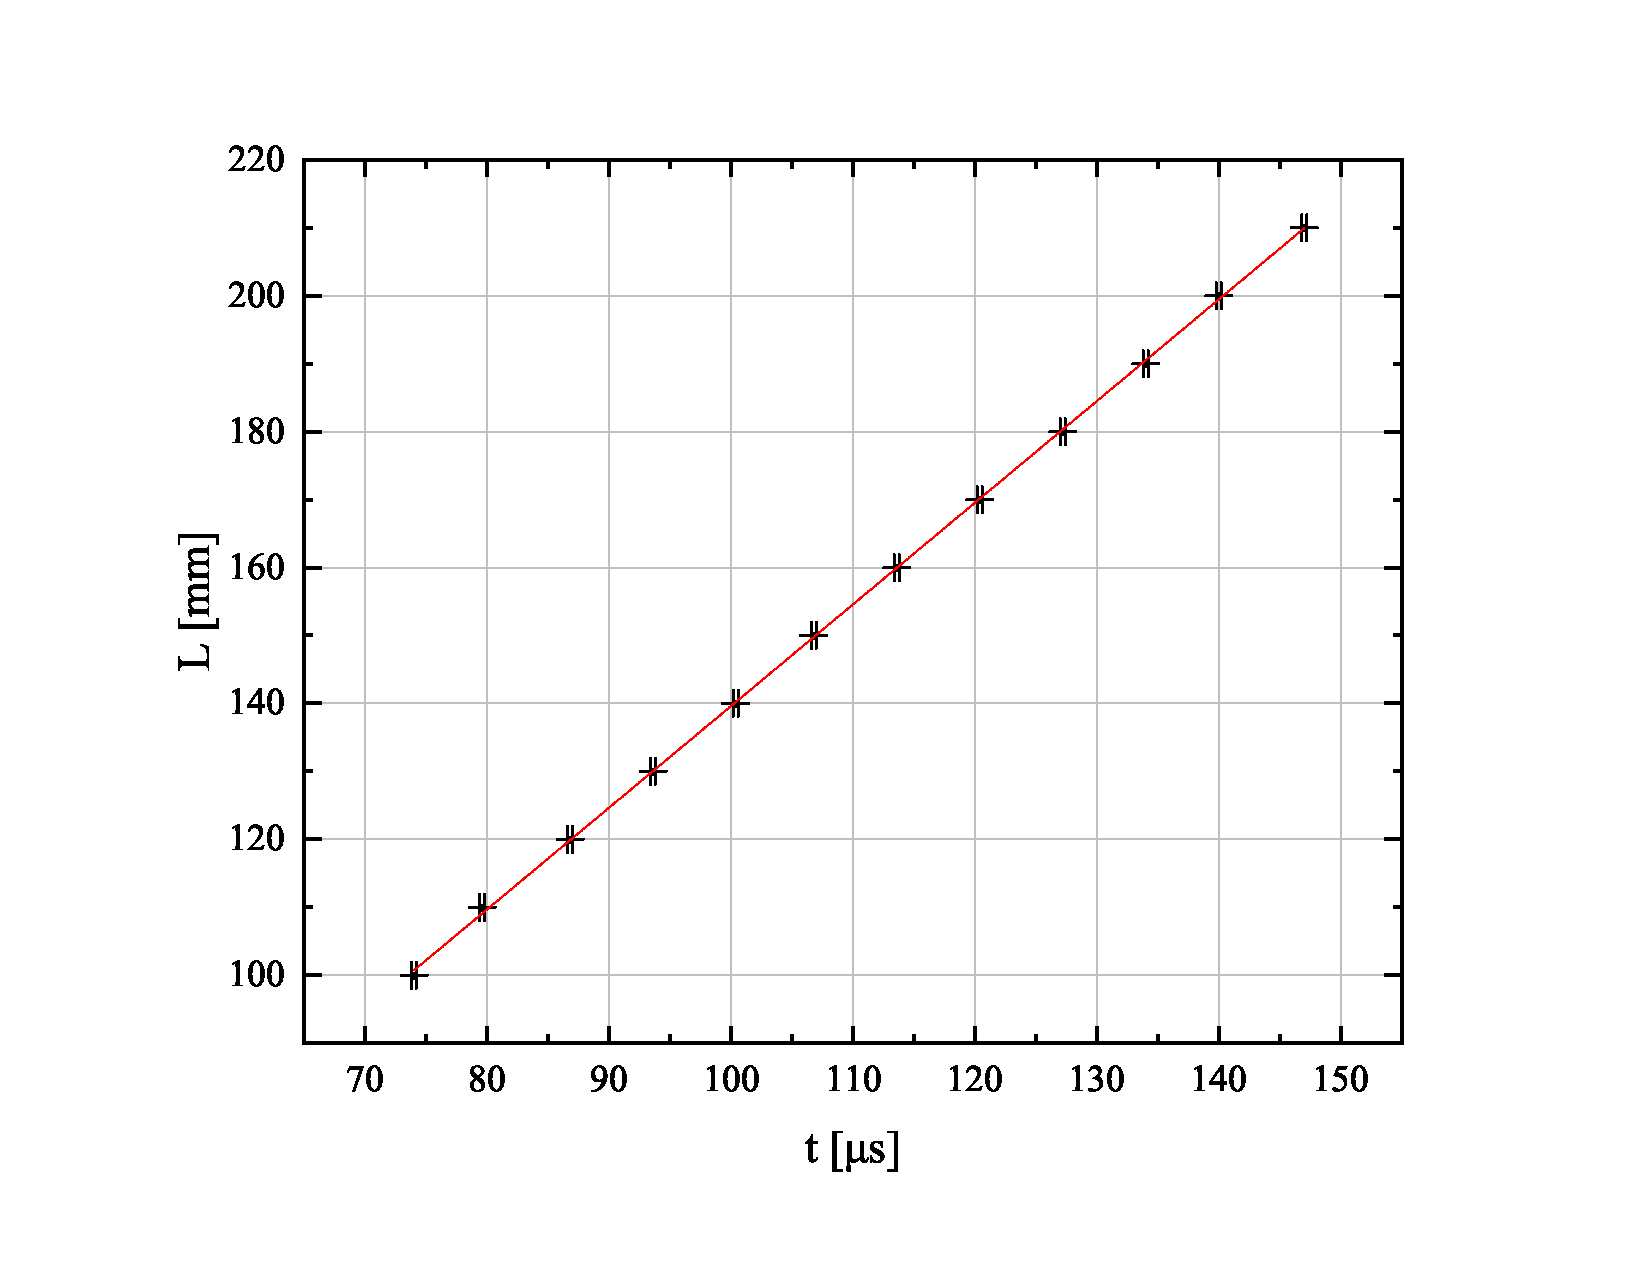
\includegraphics[width=1\linewidth]{4.eps}
		\caption{$\theta$ vs. $\omega/\omega_0$ characteristics.}
	\end{figure}
	\begin{figure}[H]
		\centering
		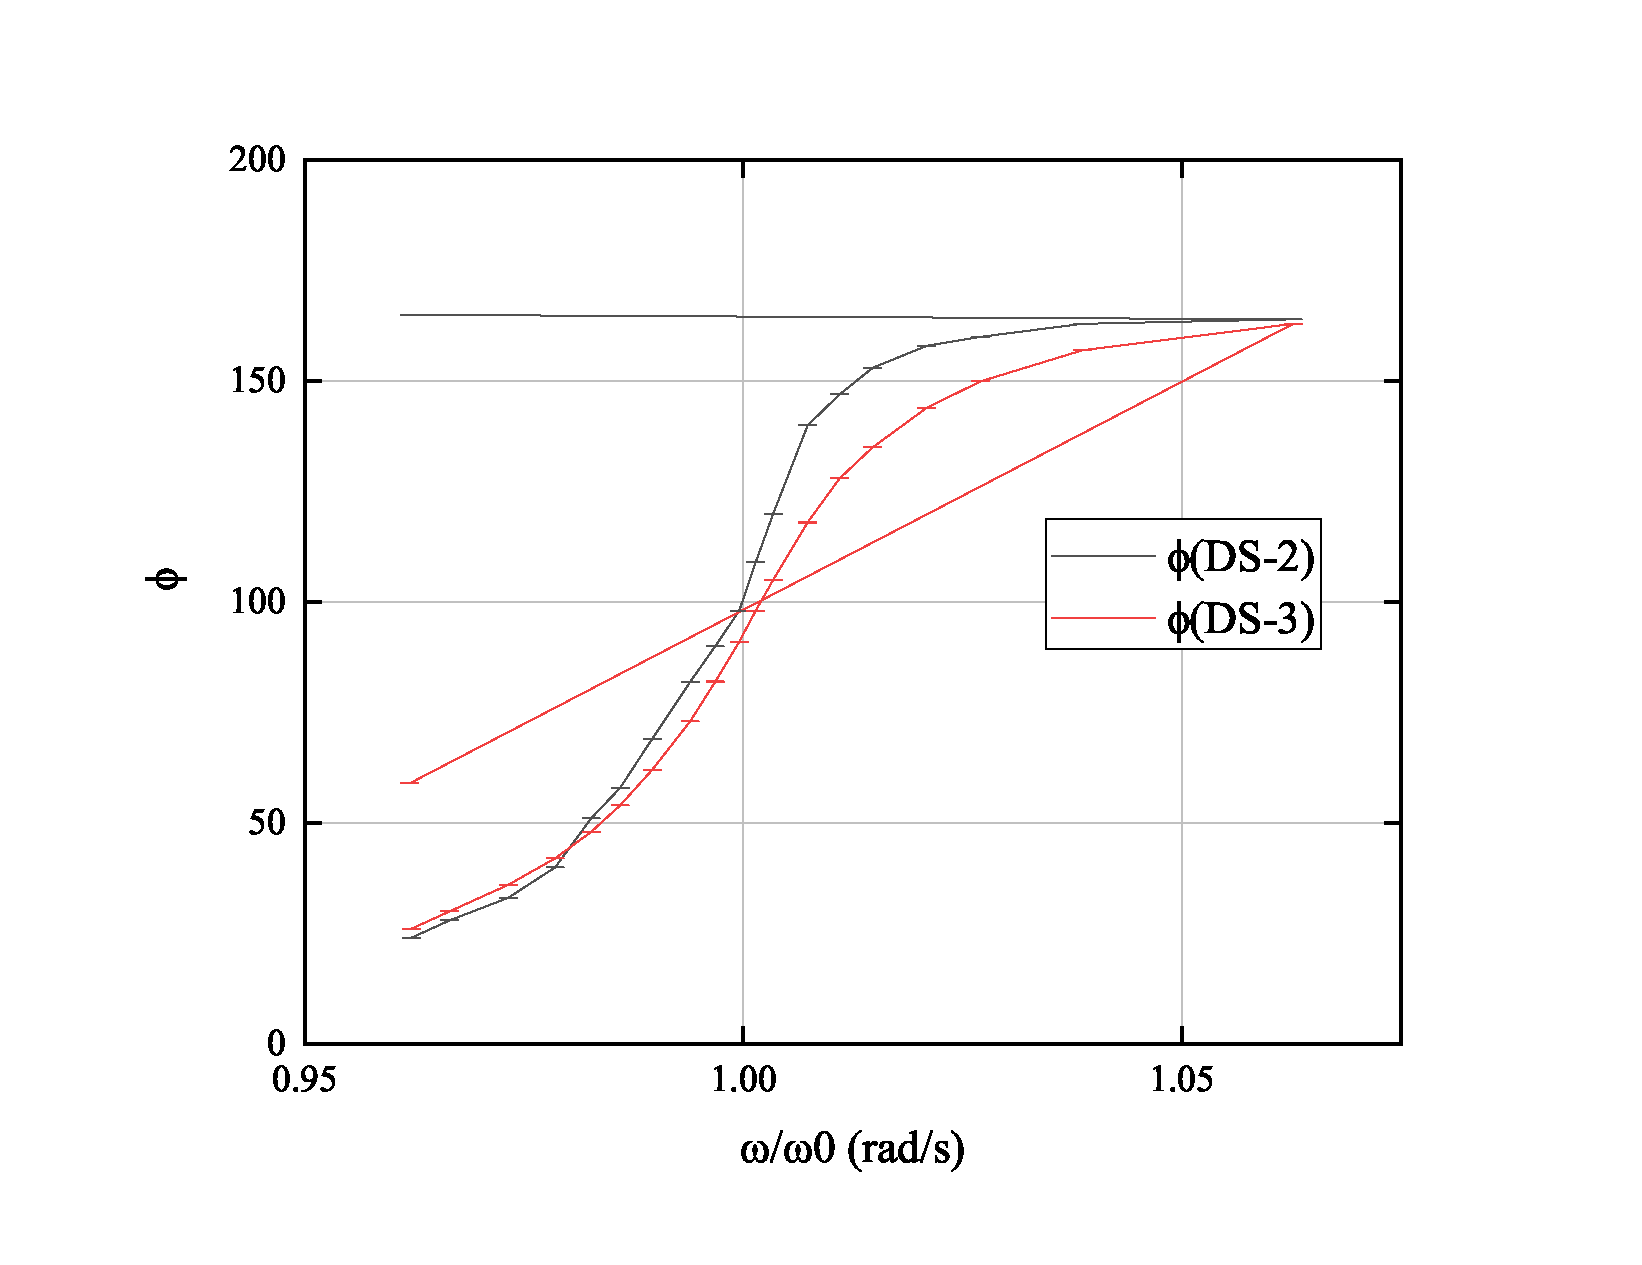
\includegraphics[width=1\linewidth]{5.eps}
		\caption{$\varphi$ vs. $\omega/\omega_0$ characteristics .}
	\end{figure}
	\section{Conclusions and discussion}
	In the experiment, we first calculate the natural angular frequency.
	\begin{equation*}
	\omega_0=3.9814\pm0.0008\ \rm{rad/s}
	\end{equation*}
	
	Then we calculate the factor $\beta$ which is the damping coefficient. Both are damping oscillations.
	\begin{equation*}
		\beta=(6.13\pm0.32)\times10^{-2}\ \rm s^{-1}
	\end{equation*}
	
	Finally, we study the driven oscillations based on the natural angular frequency we derived before and get the relationshp between the ratio $\frac{\omega}{\omega_0}$ and $\theta$ and $\varphi$. We note that the more damping coefficient, the more the ratio of the resonance and the natural frequency. Besdies, the more the phase shift, the more ratio $\frac{\omega}{\omega_0}$ and $\theta$ and $\varphi$. Taking damping into consideration, comparing the damping selection 2 and 3, we find that the higher the damping coefficient, the more the slope of the curve.

	When it comes to the control of errors, we try to accurately read and record the readings carefully. Besides, since the reading of the phase shift is not steady, the reading of the phase shift may not be very accurate.
	
	A more obvious thing is that when the angle is far from 90 degrees and near to 0 or 180 degrees, the two flashes varies more than when the angle is around 90 degrees. Sometimes, the difference between two readings can be more than 3 degrees. We just take the average of the two readings approximately and repeatedly to possibly narrow the width.
	\newpage
	\renewcommand\thesection{\Alph{section}}
	\setcounter{section}{0}
	\section{Measurement uncertainty analysis}
	\iffalse\renewcommand{\thesubsection}{\arabic{subsection}}
	\titleformat{\subsection}{\raggedright\large\bfseries}{WS-\thesubsection\enspace}{0pt}{}
	\subsection{Natural Angular Frequency}
	The uncertainty for ten periods is found first. Then the result for the natural frequency is given alon with its uncertainty.
	
	The type-B uncertainty for $T_10$ is $\Delta_{T_{10}},B=0.001$ s. To find the type-A uncertainty, we first find the standard deviation
	\begin{equation*}
	s_{T_{10}}=\sqrt{\dfrac{1}{n-1}\sum_{i=1}^n(T_{10},i-{\bar{T}_{10}})^2}=0.001915\ [\rm{s}]
	\end{equation*}
	We have $n=4$, so the type-A uncertainty $\Delta_{T_{10},A}$ is calculated as \fi
	\begin{figure}[H]
		\centering
		\includegraphics[width=1\linewidth]{6.jpg}
	\end{figure}
	\begin{figure}[H]
		\centering
		\includegraphics[width=1\linewidth]{7.jpg}
	\end{figure}
		\begin{figure}[H]
		\centering
		\includegraphics[width=1\linewidth]{8.jpg}
	\end{figure}
	\begin{figure}[H]
		\centering
		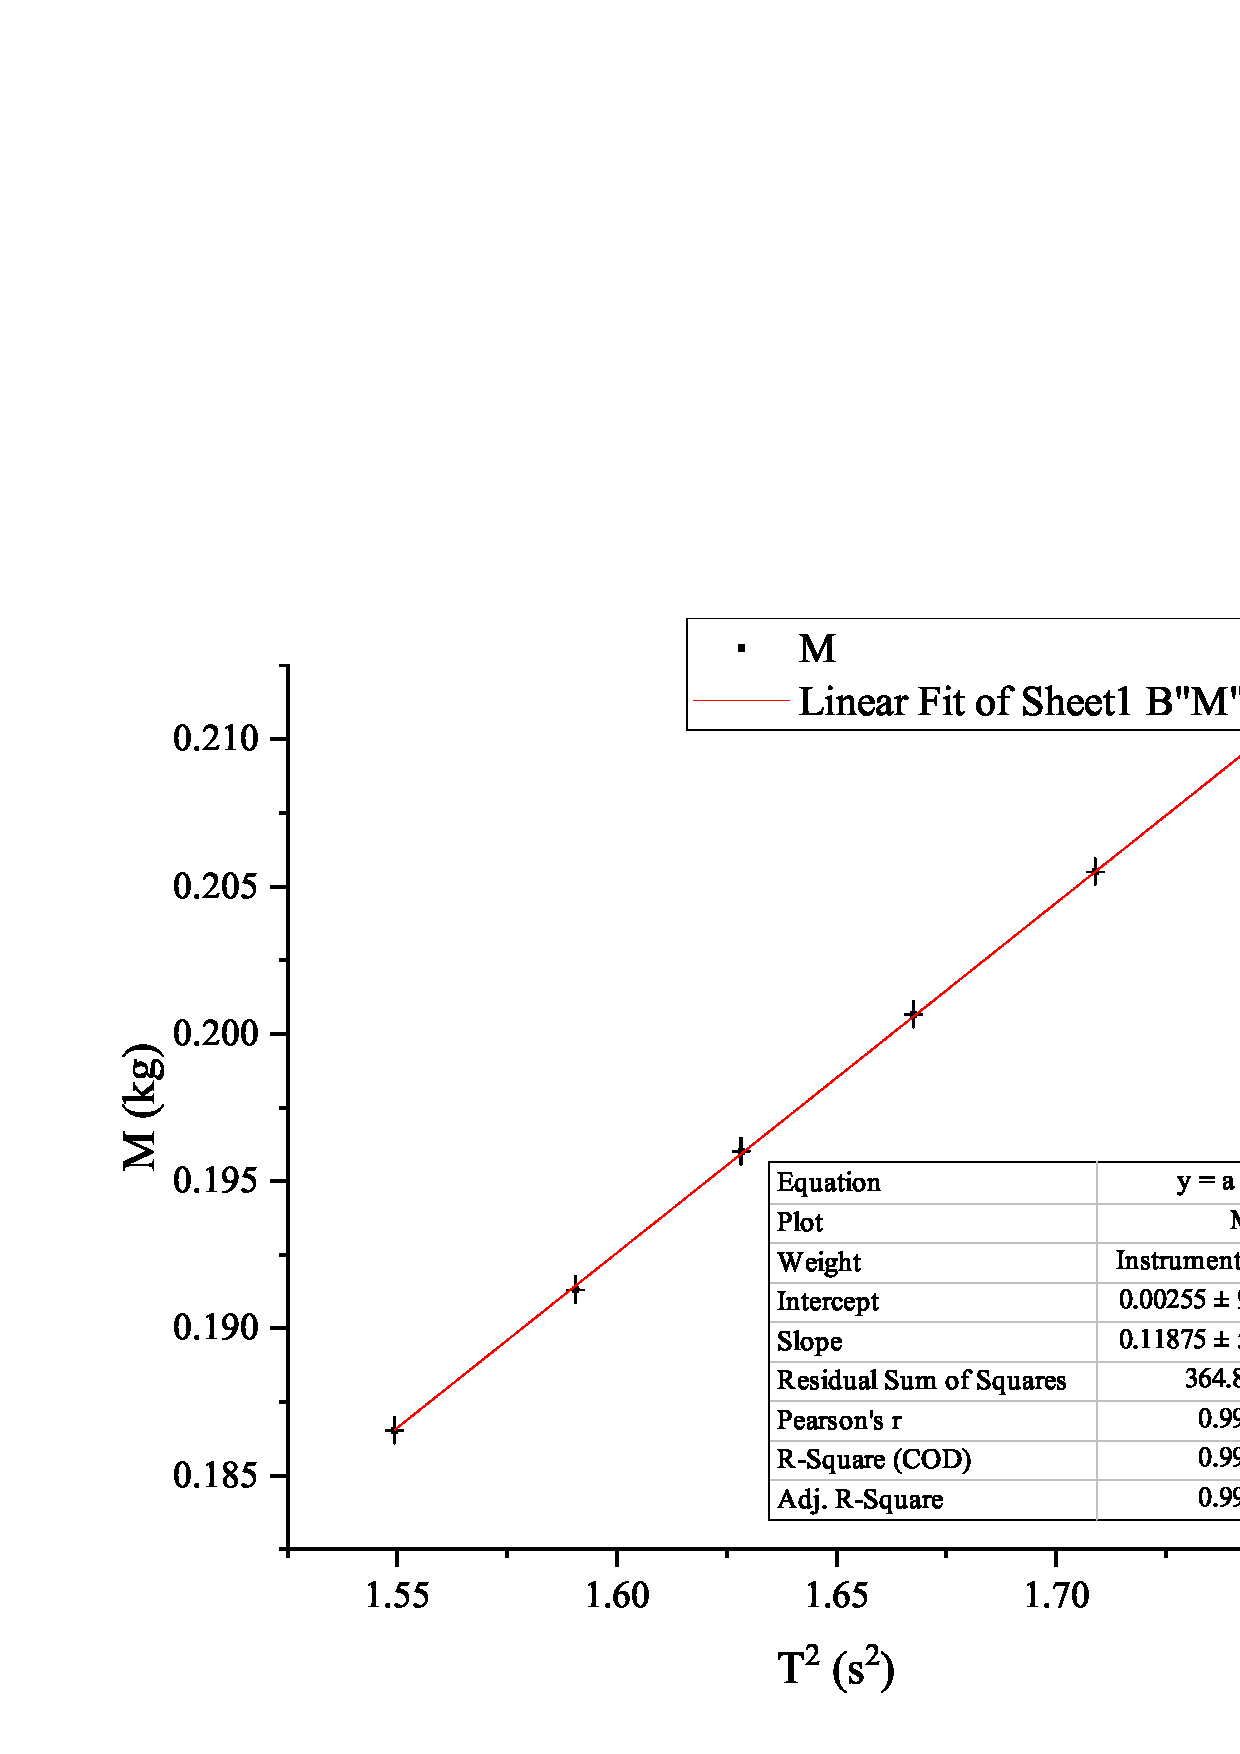
\includegraphics[width=1\linewidth]{9.jpg}
	\end{figure}
	\section{Data Sheet}
	\begin{figure}[H]
		\centering
		\includegraphics[width=1\linewidth]{10.jpg}
	\end{figure}
	\begin{figure}[H]
		\centering
		\includegraphics[width=1\linewidth]{11.jpg}
	\end{figure}
	\begin{figure}[H]
		\centering
		\includegraphics[width=1\linewidth]{12.jpg}
	\end{figure}
\end{document}